% 2003 年全国新课程理科第 16 题：正方体选项示意
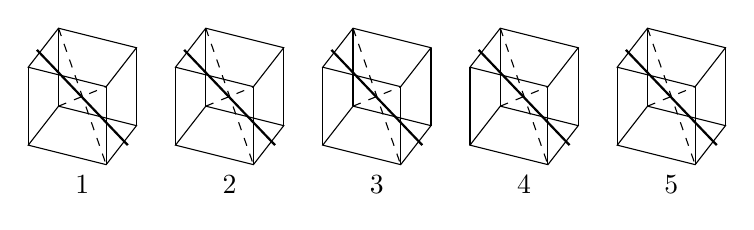
\begin{tikzpicture}[>=stealth,scale=0.55]
  \foreach \sx/\lab in {0/1,3.4/2,6.8/3,10.2/4,13.6/5}
  {
    \begin{scope}[shift={(\sx,0)}]
      \draw (0,0)--(1.8,-0.45)--(2.5,0.45)--(0.7,0.9)--cycle;
      \draw (0,0)--(0,1.8) (1.8,-0.45)--(1.8,1.35)
        (2.5,0.45)--(2.5,2.25) (0.7,0.9)--(0.7,2.7);
      \draw (0,1.8)--(1.8,1.35)--(2.5,2.25)--(0.7,2.7)--cycle;
      \draw[dashed] (0.7,0.9)--(1.8,1.35) (0.7,2.7)--(1.8,-0.45);
      \draw[thick] (0.2,2.2)--(2.3,0.0);
      \node at (1.25,-0.9) {\lab};
    \end{scope}
  }
\end{tikzpicture}
